\documentclass[conference,a4paper]{IEEEtran}

\IEEEoverridecommandlockouts

% ---- Lingua e codifica ----
\usepackage[utf8]{inputenc}
\usepackage[T1]{fontenc}
\usepackage[italian]{babel}

% ---- Matematica e riferimenti ----
\usepackage{cite}
\usepackage{amsmath,amssymb}
\usepackage[hidelinks]{hyperref}
\usepackage{url}

% ---- Figure e tabelle ----
\usepackage{graphicx}
\usepackage{placeins}
\usepackage{booktabs,array,tabularx}
\usepackage{xcolor}

% ---- Diagrammi ----
\usepackage{tikz}
\usetikzlibrary{arrows.meta,positioning,fit,backgrounds}

% ---- Configurazione ----
\graphicspath{{figures/}}

\newcommand{\code}[1]{\texttt{#1}}
\newcolumntype{Y}{>{\raggedright\arraybackslash}X}

\setlength{\emergencystretch}{1em}

\hypersetup{
    pdftitle={
        Continuum Simulator:
        monitoraggio ambientale e aggregazione distribuita Edge-Cloud
    },
    pdfauthor={Alessandro Vassallo},
    pdfsubject={Relazione progetto A2},
    pdfkeywords={
        compute continuum,
        Go,
        Kafka,
        Edge-Cloud,
        scalabilità
    }
}

% ---- Titolo ----
\title{
    Continuum Simulator: monitoraggio ambientale\\
    e aggregazione distribuita Edge--Cloud
}

\author{
    \IEEEauthorblockN{
        Alessandro Vassallo -- Matricola 0366572
    }
    \IEEEauthorblockA{
        Università degli Studi di Roma Tor Vergata\\
        Sistemi Distribuiti e Cloud Computing -- A.A. 2025/26
    }
}

\begin{document}

\pagestyle{plain}

\maketitle
\thispagestyle{plain}

\begin{abstract}
Questa relazione presenta un'applicazione distribuita sviluppata in Go
per il monitoraggio ambientale nel compute continuum. Il sistema riproduce
misure reali derivate da Sensor.Community e distribuisce l'elaborazione
tra livelli Edge e Cloud mediante MQTT e Apache Kafka. La soluzione adotta
un'aggregazione gerarchica basata su finestre temporali e un livello Cloud
scalabile orizzontalmente tramite partizionamento Kafka e consumer group.
La valutazione sperimentale analizza il comportamento del sistema al variare
del numero di Cloud Worker e delle condizioni di comunicazione.
\end{abstract}


\section{Introduzione}
\label{sec:introduzione}

L'obiettivo del progetto è lo sviluppo di un'applicazione distribuita
nel compute continuum per il monitoraggio di misure ambientali, distribuendo
l'elaborazione tra livelli Edge e Cloud. Il caso di studio utilizza dati
provenienti da sensori BME280 del dataset pubblico Sensor.Community, relativi
a temperatura, umidità e pressione e raccolti nel mese di gennaio 2025.

Il dataset storico viene utilizzato per simulare un sistema di monitoraggio
continuo. Le osservazioni vengono riprodotte preservandone le distanze
temporali in event time mediante un replay accelerato e inviate ai rispettivi
Edge Site. Ciascun Edge esegue una prima fase di validazione e aggregazione
locale, mentre il livello Cloud combina successivamente i risultati provenienti
dalle diverse zone per ottenere una vista complessiva del sistema. Questa
suddivisione permette di distribuire la computazione lungo il continuum e di
ridurre il numero di record trasferiti verso il Cloud, inoltrando aggregati
locali anziché ogni singola osservazione.

Poiché il progetto è svolto individualmente, tra i requisiti alternativi
previsti dalla traccia è stata scelta la scalabilità orizzontale. La
valutazione sperimentale studia quindi il comportamento del sistema al variare
del numero di Cloud Worker, mantenendo invariato il workload, e analizza
inoltre l'impatto delle condizioni di rete sulla pipeline distribuita.

I componenti runtime dell'applicazione sono sviluppati in Go, containerizzati
tramite Docker e distribuiti su AWS mediante un processo di deployment
automatizzato. Il preprocessing offline del dataset è invece realizzato in
Python.
\section{Dataset e costruzione del workload}
\label{sec:dataset}

Lo scenario è stato costruito a partire dal dataset relativo ai sensori ambientali BME280. È stata considerata
la finestra temporale di gennaio 2025 e il dataset, di dimensione pari a circa
6.36 GB, è stato analizzato in modo incrementale per evitare il caricamento
completo in memoria.

Una prima fase di preprocessing ha permesso di verificare la qualità dei dati,
filtrare le osservazioni esterne alla finestra temporale e individuare i
sensori dotati di coordinate geografiche valide. Delle variabili disponibili,
le coordinate geografiche sono state utilizzate per la costruzione della
topologia, mentre temperatura, umidità e pressione sono state mantenute come
misure da riprodurre durante l'esecuzione. Le variabili relative all'altitudine
e alla pressione al livello del mare, completamente prive di valori, sono state
escluse.

Lo studio è stato limitato all'area europea. Per ogni sensore è stata
determinata una posizione rappresentativa e le coordinate geografiche
WGS84 sono state proiettate nel sistema metrico EPSG:3035, in modo da
applicare il clustering su distanze spaziali coerenti. La popolazione
risultante comprende 5102 sensori europei localizzabili.

La suddivisione in Edge Site è stata ottenuta tramite K-Means sulle coordinate
proiettate. Sono stati valutati valori di $k$ compresi tra 5 e 15 utilizzando
il Silhouette Score come criterio principale di selezione, affiancato
dall'inertia e dal raggio massimo dei cluster come indicatori diagnostici.
La configurazione selezionata è risultata $k=13$, con Silhouette Score pari
a circa 0.521; l'elbow method individua invece $k=9$, utilizzato solamente
come riferimento diagnostico.

\begin{figure}[H]
    \centering
    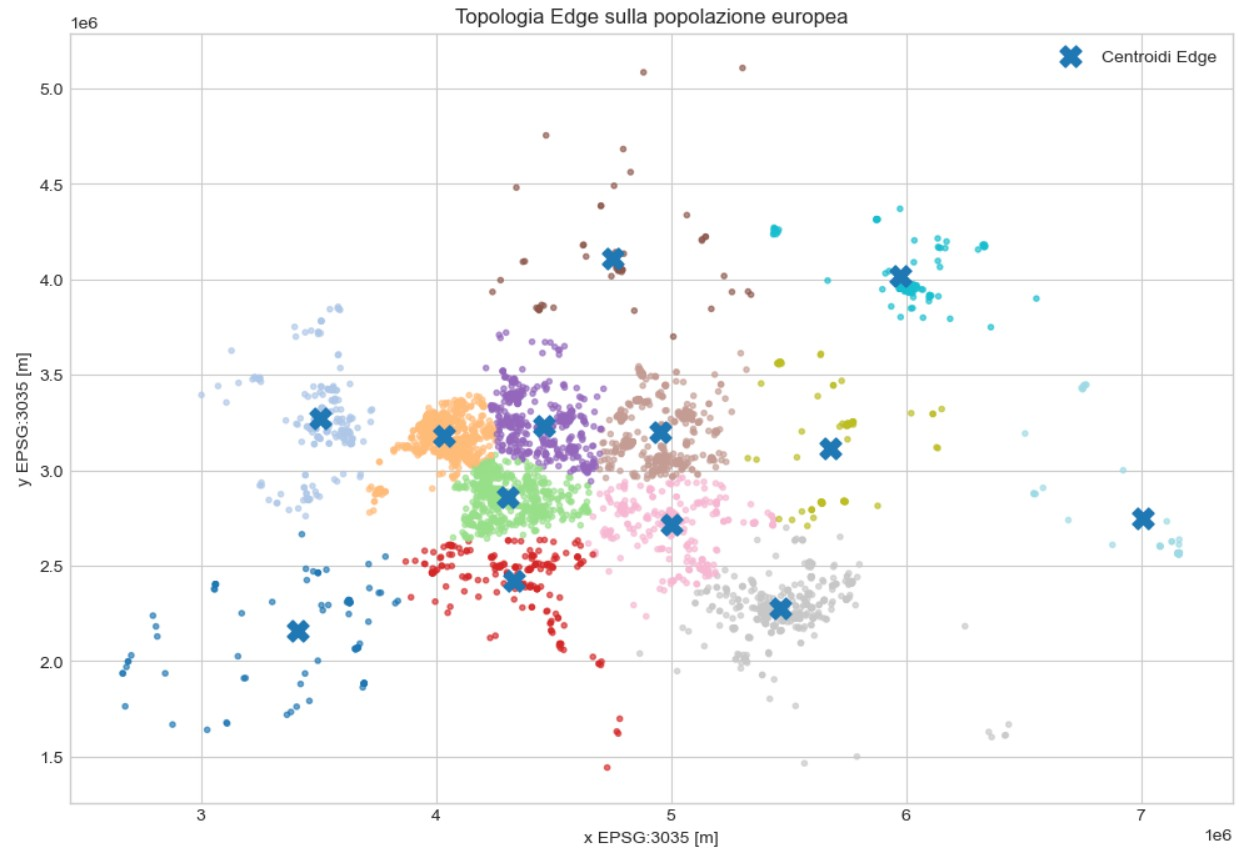
\includegraphics[width=\columnwidth]{figures/topologia_edge.jpg}
    \caption{Topologia geografica della popolazione europea e centroidi dei
    13 Edge Site.}
    \label{fig:edge-topology}
\end{figure}

Una volta determinata la topologia sull'intera popolazione europea, è stato
costruito il workload sperimentale selezionando 150 sensori. I sensori sono
stati distribuiti nel modo più uniforme possibile tra i 13 Edge Site
(11--12 sensori per Edge). La selezione all'interno di ciascun Edge è stata
effettuata utilizzando un seed pseudo-casuale fissato.
In questo modo ciascun Edge partecipa agli esperimenti con un numero
comparabile di sensori, pur mantenendo le differenze naturali nel tasso di
generazione degli eventi.

Infine, la fase di preprocessing produce due tipi di artefatti utilizzati
durante l'esecuzione: il file di topologia, che associa i sensori selezionati
agli Edge Site, e 13 shard di replay, uno per ciascun Edge, contenenti
identificativo del sensore, timestamp, pressione, temperatura e umidità.
\section{Architettura e scelte progettuali}
\label{sec:architettura}
\subsection{Flusso dei dati e responsabilità}
La Fig.~\ref{fig:architecture} rappresenta la pipeline. Ciascun sito comprende
un broker Mosquitto e un Edge Gateway; il Simulator corrispondente pubblica
JSON sul topic MQTT \code{sensors/<sensorID>/telemetry}. Il gateway valida le
misure e genera un \code{EdgeAggregate} per zona e finestra non vuota di cinque
minuti. Il record contiene eventi, conteggi validi e non validi, somma, media,
minimo e massimo per ciascuna grandezza.

\begin{figure}[t]
\centering
\begin{tikzpicture}[
  node distance=4mm,
  box/.style={draw,rounded corners=1pt,align=center,text width=6.8cm,
    minimum height=7mm,font=\footnotesize,inner sep=3pt},
  flow/.style={-{Latex[length=1.8mm]},semithick}]
\node[box,fill=gray!7] (sim) {13 Simulator: replay di 150 sensori};
\node[box,below=of sim,fill=blue!6] (edge) {13 siti Edge: Mosquitto + Gateway\\
  aggregazione locale 5 min e watermark per Edge};
\node[box,below=of edge] (k1) {Kafka: \texttt{edge-aggregates}\\6 partizioni, chiave \texttt{edge\_id}};
\node[box,below=of k1,fill=orange!9] (workers) {$W$ Cloud Worker, stesso consumer group\\
  finestre 15 min, minimo dei watermark per partizione};
\node[box,below=of workers] (k2) {Kafka: \texttt{cloud-partition-aggregates}\\
  1 partizione fisica, 6 sorgenti logiche};
\node[box,below=of k2,fill=orange!9] (global) {Global Aggregator\\
  riduzione degli stessi intervalli di 15 min};
\node[box,below=of global,fill=gray!7] (sink) {Sink: log JSON oppure PostgreSQL};
\foreach \a/\b in {sim/edge,edge/k1,k1/workers,workers/k2,k2/global,global/sink}
  \draw[flow] (\a) -- (\b);
\end{tikzpicture}
\caption{Architettura logica. I due topic risiedono sullo stesso broker Kafka.
Le repliche dei worker non modificano le sei sorgenti logiche del Global.}
\label{fig:architecture}
\end{figure}

Kafka disaccoppia la produzione Edge dal consumo Cloud e mantiene i record in
un log persistente~\cite{kafka}. Il topic \code{edge-aggregates} ha sei
partizioni. La chiave \code{edge\_id} e il partizionatore hash mantengono
\code{EdgeAggregate}, \code{EdgeWatermark} e marker terminale dello stesso
Edge nella medesima partizione e nello stesso ordine. Il numero di partizioni
e la membership degli Edge rimangono invariati per l'intera run.

I Cloud Worker condividono un consumer group: ciascuna partizione è assegnata
a un solo membro del gruppo. La topologia Edge è proiettata sulle partizioni
con lo stesso hash del producer; ogni worker mantiene uno stato separato per
ciascuna partizione assegnata, indipendente dalla propria identità. I contributi
Edge sono combinati su finestre di quindici minuti. Gli output sono
\code{CloudPartitionAggregate}, identificati da partizione sorgente e confini
temporali, pubblicati sul secondo topic Kafka. Il Global Aggregator combina i
partial con la stessa coppia di confini e produce il risultato nel sink.

\subsection{Aggregazione componibile}
Per una metrica $m$, ogni aggregato conserva il numero di misure valide $n_m$,
il numero di misure non valide $u_m$ e la somma $s_m$, oltre agli estremi.
La combinazione di contributi disgiunti $j$ applica
\begin{equation}
n_m=\sum_j n_{m,j},\qquad u_m=\sum_j u_{m,j},\qquad
s_m=\sum_j s_{m,j}.
\end{equation}
La media si ottiene da $s_m/n_m$ se $n_m>0$; altrimenti media ed estremi sono
nulli. Minimo e massimo si combinano considerando soltanto contributi validi.
La somma dei conteggi validi e non validi deve coincidere con il numero di
eventi dell'aggregato per ciascuna metrica.

Conservare la somma evita la media non pesata delle medie locali, che sarebbe
errata in presenza di numerosità differenti. L'operazione è componibile in
aritmetica esatta; con valori floating point l'equivalenza numerica va
verificata con una tolleranza. I cinque minuti Edge dividono esattamente i
quindici minuti Cloud, per cui ogni aggregato locale appartiene a una sola
finestra Cloud. Un aggregato che attraversa un confine Cloud viene rifiutato.

\subsection{Progresso, contributi vuoti e completamento}
L'Edge mantiene una finestra corrente in event time. L'arrivo di un evento
della finestra successiva determina la pubblicazione della precedente, seguita
da \code{EdgeWatermark(e,t)}. Tale controllo certifica che l'Edge $e$ non
pubblicherà successivamente aggregati con \code{window\_end} minore o uguale
a $t$. Il watermark è monotono. L'EOS ricevuto dal Simulator chiude l'ultima
finestra; dopo averne completato la scrittura Kafka, l'Edge pubblica il distinto
marker \code{EdgeEndOfInput}. Gli eventi appartenenti a finestre già chiuse
sono scartati e conteggiati; il contratto richiede shard ordinati temporalmente.

Una partizione Cloud può contenere Edge con velocità differenti. Il worker
memorizza, per ogni Edge atteso nella partizione $P$, il watermark
$W_e$ e il flag terminale. Finché un Edge attivo non ha prodotto un watermark,
non è possibile certificarne il progresso. La frontiera locale è
\begin{equation}
W_P=\min_{e\in E_P,\ e\ \mathrm{attivo}} W_e .
\end{equation}
Solo le finestre con fine non successiva a $W_P$ sono definitive. Un Edge
terminato non partecipa più al minimo; la cessazione temporanea del traffico,
invece, non equivale alla conclusione della sorgente.

Il worker pubblica prima i partial definitivi e poi il controllo di progresso
\code{PartitionProgress(P,t)}, con $t=W_P$. Quando tutti gli Edge di $P$ terminano,
pubblica in ordine gli ultimi partial e infine \code{PartitionEndOfReplay(P)};
una partizione senza Edge produce direttamente tale controllo. Un aggregato
ricevuto dietro un watermark già certificato viola il protocollo e invalida la
run: una finestra emessa non viene riaperta. L'ordine fra dati e controlli
permette una rappresentazione sparsa: l'assenza di un partial, dopo il relativo
progresso o EOS, equivale a un contributo zero.

È stata considerata anche un'alternativa in cui il Cloud conoscesse soltanto
le partizioni Kafka, senza la membership degli Edge, e stimasse la frontiera
come massimo event time osservato meno un ritardo. La soluzione ridurrebbe
l'accoppiamento con la topologia, ma un Edge veloce potrebbe anticipare la
chiusura rispetto a uno lento; inoltre il ritardo sarebbe un parametro euristico.
Si è quindi preferita la certificazione esplicita degli Edge e il minimo per
partizione, privilegiando la correttezza nel deployment statico adottato.

Il Global conosce soltanto le sei partizioni sorgente. Per una finestra attende
da ciascuna un partial oppure un controllo di progresso/EOS che certifichi il
contributo zero. Non introduce nuove finestre, non ricalcola watermark e non
usa timeout per dichiarare completi risultati incompleti. Il replay termina
dopo gli EOS di tutte le partizioni e l'emissione delle finestre pendenti.

\subsection{Parallelismo indipendente dal risultato}
Con $W=1,2,4,6$ cambia il numero di esecutori, non quello delle partizioni
sorgente (Tab.~\ref{tab:workers}). Anche con un solo worker la pipeline passa
dal secondo topic e dal Global. In presenza di dati in tutte le partizioni si
producono sei partial per finestra; in caso contrario alcuni contributi sono
certificati come zero. Il Global non aggrega per identità del worker.

\begin{table}[t]
\caption{Distribuzione bilanciata delle sei partizioni. L'assegnazione
effettiva degli identificativi è decisa dal consumer group.}
\label{tab:workers}
\centering
\begin{tabular}{ccc}
\toprule
Worker & Partizioni per worker & Sorgenti logiche Global\\
\midrule
1 & 6 & 6\\
2 & 3, 3 & 6\\
4 & 2, 2, 1, 1 & 6\\
6 & 1, 1, 1, 1, 1, 1 & 6\\
\bottomrule
\end{tabular}
\end{table}

Ogni worker usa letture concorrenti ma un solo ciclo di elaborazione; il
parallelismo computazionale cresce quindi tramite processi aggiuntivi. Sei
partizioni costituiscono il limite del parallelismo utile del gruppo. La
distribuzione delle partizioni non garantisce un uguale costo: il numero di
Edge e il volume dei loro aggregati possono differire. Il broker condiviso e
il Global restano inoltre possibili colli di bottiglia.

\section{Implementazione}
\label{sec:implementazione}

\subsection{Aggregazione Edge e Cloud}

L'elaborazione utilizza finestre tumbling basate sull'event time. Ciascun
Edge mantiene una finestra corrente e assegna ogni evento alla finestra
determinata dal relativo timestamp. Per ogni grandezza ambientale vengono
mantenuti il numero di valori validi e non validi, la somma, il minimo e il
massimo. Al momento della chiusura della finestra viene inoltre calcolata la
media sui soli valori validi.

Le statistiche sono state scelte in modo da poter essere combinate nei
livelli successivi senza conservare le singole osservazioni. Indicando con
$n_j$ il numero di valori validi e con $s_j$ la loro somma nel contributo
$j$, la combinazione di più aggregati utilizza

\begin{equation}
    n = \sum_j n_j,
    \qquad
    s = \sum_j s_j,
    \qquad
    \bar{x} = \frac{s}{n}.
\end{equation}

Minimo e massimo globali sono ottenuti rispettivamente come minimo e massimo
dei contributi che contengono almeno un valore valido. In questo modo la media
globale non viene calcolata come media delle medie locali, che produrrebbe un
risultato errato quando gli aggregati contengono numerosità differenti.

Le finestre Cloud hanno durata configurabile, ma devono essere un multiplo
intero della durata delle finestre Edge. Ogni \code{EdgeAggregate} appartiene
quindi interamente a una sola finestra Cloud. I Cloud Worker combinano gli
aggregati ricevuti per partizione Kafka e producono un
\code{CloudPartitionAggregate}; il Global Aggregator applica infine la stessa
operazione di riduzione ai contributi delle diverse partizioni relativi allo
stesso intervallo temporale.

\subsection{Progresso event-time e completamento}

La chiusura delle finestre Cloud è governata dal progresso in event time
delle sorgenti e non da timeout in processing time. Ogni
\code{EdgeAggregate} contiene il campo \code{CompleteThrough}, che certifica
che l'Edge non produrrà successivamente aggregati con fine della finestra
precedente o uguale a tale istante.

Quando l'arrivo di un evento determina il passaggio a una nuova finestra,
l'Edge emette l'aggregato della finestra precedente e può avanzare
\code{CompleteThrough} fino all'inizio della nuova finestra. In questo modo
vengono certificate anche eventuali finestre intermedie prive di eventi.
Gli Edge non producono infatti aggregati espliciti per le finestre vuote.

Il Cloud mantiene separatamente il progresso di ciascun Edge appartenente
alla partizione Kafka elaborata. Indicando con $C_e$ il valore
\code{CompleteThrough} dell'Edge attivo $e$ e con $S$ il massimo disallineamento
ammesso tra le sorgenti, la frontiera della partizione è determinata da

\begin{equation}
W_P =
\max\left(
    \min_{e \in E_P} C_e,\;
    \max_{e \in E_P} C_e - S
\right).
\end{equation}

Finché almeno un Edge attivo non ha ancora comunicato il proprio progresso,
la frontiera non può avanzare. In condizioni normali essa coincide quindi
con il minimo progresso degli Edge della partizione; il secondo termine
impedisce invece che una sorgente eccessivamente in ritardo blocchi
indefinitamente la finalizzazione delle finestre. Una finestra Cloud viene
emessa quando il proprio estremo superiore non è successivo a $W_P$.

Un aggregato relativo a una finestra già superata dalla frontiera è
considerato \emph{late}: non modifica né riapre il risultato già emesso.
Il progresso contenuto nel record può comunque essere utilizzato per
aggiornare lo stato dell'Edge e consentirgli di riallinearsi alle altre
sorgenti.

Poiché il workload è ottenuto dal replay di un dataset finito, è inoltre
necessario determinare esplicitamente la conclusione del flusso. Al termine
del proprio replay ciascun Simulator invia un marker di fine input al
rispettivo Edge. L'Edge pubblica l'ultima finestra ancora aperta e,
successivamente, un \code{EdgeEndOfInput}. Quando tutti gli Edge appartenenti
a una partizione sono terminati, il Cloud Worker emette gli eventuali
aggregati ancora pendenti e infine un \code{PartitionEndOfReplay}.

Il Global Aggregator utilizza i risultati delle partizioni insieme ai relativi
progressi e marker terminali per distinguere un contributo non ancora arrivato
da un contributo effettivamente assente. Una finestra globale può quindi
essere prodotta quando, per ogni partizione sorgente, è disponibile il
relativo aggregato oppure è stato certificato che non ne verranno prodotti
altri per quell'intervallo. Il replay termina quando tutte le partizioni hanno
raggiunto lo stato terminale e non rimangono finestre pendenti.

\subsection{Comunicazione e affidabilità}

La comunicazione tra Simulator ed Edge utilizza MQTT. Gli eventi dei sensori
sono serializzati in JSON e pubblicati con QoS~0. JSON è stato scelto in
questo tratto della pipeline per la semplicità della rappresentazione e per
la facilità con cui i messaggi possono essere ispezionati durante lo sviluppo
e il debugging. La telemetria viene inoltre prodotta con frequenza elevata:
l'utilizzo di QoS~0 evita di attendere una conferma per ogni singola
osservazione e permette al replay di procedere secondo il rate configurato.
Il marker di fine replay utilizza invece QoS~1 e viene considerato completato
soltanto dopo la ricezione del relativo PUBACK, poiché la sua perdita
impedirebbe di determinare correttamente la terminazione della sorgente.

La comunicazione tra Edge e Cloud e tra Cloud Worker e Global Aggregator è
invece affidata ad Apache Kafka. In questo tratto i messaggi sono serializzati
in formato Apache Avro. Rispetto al JSON, Avro fornisce una rappresentazione
binaria più compatta e definisce esplicitamente la struttura e i tipi dei
record scambiati, caratteristica utile per aggregati composti da numerosi
campi numerici e temporali. Gli schemi Avro sono inclusi direttamente
nell'applicazione e devono quindi essere condivisi in modo coerente da
producer e consumer; non viene utilizzato uno Schema Registry.

Il tipo logico di ciascun record Kafka è indicato mediante l'header
\code{record\_type}. In questo modo lo stesso meccanismo di trasporto può
veicolare aggregati, informazioni di progresso e marker terminali. Questi
ultimi non richiedono dati applicativi e vengono pertanto inviati con payload
vuoto.

Gli Edge utilizzano writer Kafka sincroni con acknowledgment del broker. Gli
aggregati appartenenti allo stesso Edge e il relativo
\code{EdgeEndOfInput} sono scritti sulla medesima partizione; prima di
pubblicare il marker terminale vengono completate le scritture degli aggregati
precedenti. Analogamente, il Cloud pubblica per ciascuna partizione prima gli
eventuali \code{CloudPartitionAggregate}, quindi il relativo
\code{PartitionProgress} e infine, quando necessario,
\code{PartitionEndOfReplay}. L'ordinamento permette ai consumer downstream di
interpretare un'informazione di progresso solo dopo aver ricevuto tutti i dati
che essa certifica.

I Cloud Worker effettuano il commit degli offset Kafka solamente dopo che il
record di input è stato elaborato e gli eventuali output sono stati pubblicati
con successo. I commit possono essere raggruppati in batch configurabili per
ridurne il costo; la ricezione di un marker terminale forza invece il commit
degli offset ancora pendenti. Il Global Aggregator applica lo stesso principio,
effettuando il commit dopo l'elaborazione e la scrittura del risultato nel
sink.

Questa strategia evita di confermare un record prima che i suoi effetti siano
stati propagati, ma non realizza una transazione atomica end-to-end tra stato,
output Kafka e offset di consumo. Un arresto dopo la pubblicazione dell'output
ma prima del commit può quindi causare la rilettura di un record. Per questo
motivo gli aggregati utilizzano identificativi deterministici e i componenti
riconoscono i duplicati identici, mentre nel sink PostgreSQL l'identificativo
dell'aggregato è una chiave univoca.

\subsection{Deployment e piattaforma software}

L'applicazione è sviluppata in Go e ciascun componente principale viene
distribuito come container Docker. La configurazione del sistema è descritta
tramite file YAML, dai quali il programma \code{deploygen} genera
automaticamente i file Docker Compose necessari all'esecuzione. In questo modo
parametri quali numero di Cloud Worker, numero di partizioni Kafka, dimensione
delle finestre e parametri di batching possono essere modificati senza
intervenire sul codice applicativo.

Per il deployment distribuito l'infrastruttura AWS è definita mediante
Terraform. Sono previsti quattro host EC2 con ruoli distinti: Simulator, Edge,
Cloud Core e Workers. L'host Simulator esegue i processi di replay, l'host Edge
ospita i broker Mosquitto e gli Edge Gateway, l'host Workers esegue le repliche
dei Cloud Worker, mentre Cloud Core ospita Kafka e il Global Aggregator.
La separazione consente di far attraversare realmente la rete ai flussi
Simulator--Edge ed Edge--Cloud e di modificare indipendentemente il numero di
worker utilizzato negli esperimenti.

La persistenza dei risultati globali può essere affidata a un'istanza
PostgreSQL gestita tramite Amazon RDS. Il database non è esposto pubblicamente
ed è raggiungibile dal solo Cloud Core. L'infrastruttura, la configurazione
applicativa e l'avvio degli esperimenti sono gestiti tramite script dedicati,
in modo da rendere ripetibile la preparazione dell'ambiente e la raccolta degli
artefatti prodotti da ogni esecuzione.

Le principali librerie utilizzate dall'applicazione sono Eclipse Paho per MQTT,
\code{kafka-go} per la comunicazione con Kafka, \code{goavro} per la
serializzazione Avro e \code{pgx} per l'accesso a PostgreSQL. Il preprocessing
offline del dataset è invece realizzato in Python mediante pandas,
scikit-learn e pyproj. Non viene utilizzato un framework esterno di stream
processing: la gestione delle finestre, dello stato e del progresso event-time
è implementata direttamente nei componenti Go.
\section{Valutazione sperimentale}
\label{sec:valutazione}

\subsection{Ambiente e metodologia sperimentale}

La valutazione risponde a due domande. La prima riguarda la capacità del
livello Cloud di assorbire lo stesso workload riducendo ritardo e backlog
all'aumentare delle repliche. La seconda riguarda l'effetto di latenza e banda
disponibile sui due confini di rete Simulator--Edge ed Edge--Cloud. Le prove
sono eseguite sul deployment AWS di Fig.~\ref{fig:architecture}; ogni
configurazione viene ripetuta tre volte e viene considerata valida soltanto se
i controlli di qualità confermano la completezza della pipeline.

Il workload definitivo comprende 2\,106\,784 osservazioni distribuite tra 13
replay shard. Il replay usa un fattore di accelerazione pari a 20\,000; tale
valore è stato scelto mediante una calibrazione preliminare per esercitare il
livello Cloud senza introdurre intenzionalmente perdite nei componenti a
monte. La configurazione comune alle campagne è riassunta in
Tab.~\ref{tab:experiment-configuration}.

\begin{table}[t]
    \caption{Configurazione comune delle campagne sperimentali.}
    \label{tab:experiment-configuration}
    \centering
    \begin{tabular}{@{}lr@{}}
        \toprule
        Parametro & Valore \\
        \midrule
        Edge Site / Simulator & 13 \\
        Partizioni \code{edge-aggregates} & 6 \\
        Finestra Edge & 5 min \\
        Finestra Cloud & 15 min \\
        Fattore di accelerazione & 20\,000 \\
        Batch producer Edge & 10 \\
        Batch commit Cloud & 100 \\
        \bottomrule
    \end{tabular}
\end{table}

Per ogni run vengono conservati configurazione effettiva, log, metriche dei
container, serie temporali del consumer lag e aggregati finali PostgreSQL. La
riconciliazione verifica che gli eventi offerti dai Simulator coincidano con
quelli accettati dagli Edge, che non vi siano errori di pubblicazione o record
late, che tutte le finestre globali siano complete e che il lag finale sia
nullo. Le esecuzioni che non rispettano tali condizioni vengono documentate
ma escluse dal confronto prestazionale.

La metrica principale è la \emph{global emission latency}, cioè il ritardo con
cui una finestra globale viene emessa rispetto all'istante nominale previsto
dalla timeline accelerata. Indicando con $t_0$ l'avvio sincronizzato del
replay, con $e_0$ l'origine della timeline del dataset, con $f$ il fattore di
accelerazione e con $w_e$ la fine della finestra, la deadline nominale è

\begin{equation}
    d(w_e) = t_0 + \frac{w_e-e_0}{f}.
\end{equation}

La latenza è la differenza tra l'istante di emissione del Global Aggregator e
$d(w_e)$. Vengono riportati media, mediana, 95-esimo e 99-esimo percentile,
insieme al massimo consumer lag, all'utilizzo di CPU e memoria e al tempo
complessivo della run. Poiché il replay impone il ritmo di ingresso, il
makespan e il goodput sono usati soprattutto come controlli di capacità e
completezza; latenza e backlog evidenziano più direttamente il beneficio del
parallelismo Cloud.

\subsection{Scalabilità del livello Cloud}

La campagna usa un fixed workload e varia il numero di Cloud Worker tra
$W\in\{1,2,3,4,6\}$. Il topic mantiene sei partizioni in tutte le prove:
in questo modo cambia soltanto il numero di partizioni elaborate in parallelo,
mentre restano invariati dati, assegnamento degli Edge e risultati attesi. Sei
worker costituiscono il limite di parallelismo utile della configurazione;
repliche ulteriori rimarrebbero senza partizioni assegnate.

Il confronto utilizza le distribuzioni della global emission latency, il picco
e l'evoluzione del lag per partizione e l'utilizzo delle risorse. I valori
riportati nei grafici saranno la media delle tre repliche valide; la
variabilità tra run verrà mostrata esplicitamente, senza interpretare come
speedup la sola durata del replay, che è principalmente determinata dal rate
di ingresso.

% Risultati da inserire al termine della campagna:
% - tabella con run valide/scartate e motivazione;
% - grafico p50/p95/p99 della global emission latency per W;
% - grafico del massimo lag Cloud per W e, se utile, serie temporali W1/W6;
% - CPU dei worker e del Cloud Core;
% - discussione dello sbilanciamento fra le sei partizioni e del punto di
%   saturazione oltre il quale aggiungere worker non porta benefici.

\subsection{Impatto delle condizioni di rete}

Le condizioni di rete vengono emulate tramite Linux \code{tc-netem} nel
network namespace dei container interessati. Le regole sono selettive: sul
confine Simulator--Edge agiscono soltanto sul traffico MQTT verso il broker
associato; sul confine Edge--Cloud agiscono soltanto sulle connessioni Kafka.
Il traffico di orchestrazione e raccolta delle metriche non viene quindi
alterato.

La campagna usa tre Cloud Worker e confronta una baseline senza emulazione con
ritardi aggiuntivi di 50 e 100 ms e con limiti di banda applicati separatamente
ai due confini. Ogni profilo modifica una sola variabile alla volta. Oltre alla
latenza di emissione e al lag vengono controllati code, errori e perdite: una
riduzione apparente del carico ottenuta scartando telemetria non viene
interpretata come miglioramento prestazionale.

% Risultati da inserire al termine della campagna:
% - tabella con profilo, run valide, latenza e banda effettivamente applicate;
% - grafici latency/lag rispetto al ritardo e al rate sui due confini;
% - confronto delle code Simulator/Edge e dei tempi di pubblicazione Kafka;
% - distinzione fra degradazione controllata e perdita di completezza.

\subsection{Discussione dei risultati}

La discussione finale confronterà i benefici dell'aumento dei worker con i
limiti osservati: parallelismo massimo pari al numero di partizioni,
sbilanciamento residuo del carico, costo del coordinamento tramite Kafka e
possibile contesa del Cloud Core, che ospita broker e Global Aggregator. Le
conclusioni distingueranno inoltre la capacità di mantenere risultati completi
dalla sola velocità di elaborazione.

% Completare dopo le campagne con conclusioni quantitative, evitando di
% generalizzare oltre il deployment e il dataset effettivamente misurati.

\section{Limitazioni}
\label{sec:limitazioni}

\subsection{Scalabilità durante l'esecuzione}

I Cloud Worker e il Global Aggregator mantengono in memoria lo stato delle
finestre in elaborazione. Tale stato non viene migrato tra Worker e non è
previsto un meccanismo di checkpoint che consenta di trasferirlo durante una
run.

Per questo motivo la scalabilità viene valutata configurando il numero di
Cloud Worker prima dell'avvio del replay e confrontando esecuzioni distinte.
Un rebalance del consumer group dopo l'inizio dell'elaborazione invalida la
run e i Worker non riprendono una precedente esecuzione a partire da offset
già committati. Il sistema permette quindi di studiare l'aumento del
parallelismo tra esecuzioni differenti, ma non implementa una variazione
dinamica del numero di Worker durante la stessa run.

\subsection{Completezza e rappresentatività}

La telemetria Simulator--Edge utilizza MQTT con QoS~0 e attraversa code di
capacità limitata. Per evitare che eventuali perdite vengano interpretate
come un miglioramento prestazionale, nella campagna di scalabilità vengono
considerate valide soltanto le esecuzioni che mantengono il 100\% degli
eventi, senza drop o contributi late.

Negli esperimenti bounded, invece, i contributi late costituiscono un effetto
previsto della politica event-time studiata. Una sorgente che rimane indietro
oltre lo skew configurato può essere superata dalla frontiera; i contributi
che raggiungono successivamente una finestra già finalizzata vengono
registrati come late e scartati. Eventuali drop nei Simulator, negli Edge o
nell'emulazione di rete rimangono invece condizioni di invalidità della run.

Il workload utilizza un solo tipo di dispositivo, i sensori BME280, e
considera le osservazioni relative a un solo mese. I 150 sensori selezionati
sono distribuiti in modo quasi uniforme tra i 13 Edge Site, ma il numero di
eventi prodotto dalle diverse zone non è necessariamente uniforme. Le medie
sono inoltre calcolate a partire dal numero di campioni validi, per cui
contributi contenenti un numero maggiore di osservazioni hanno un peso
maggiore nel risultato globale.

I Cloud Worker condividono il medesimo host Workers e sono eseguiti con i
limiti di CPU e memoria definiti dal profilo sperimentale. I risultati
descrivono pertanto il comportamento del deployment e del workload analizzati
e non vengono generalizzati automaticamente ad altri dataset, algoritmi più
costosi o configurazioni infrastrutturali differenti.

\section{Conclusioni}
\label{sec:conclusioni}

La campagna AWS mostra che l'aumento del parallelismo del livello Cloud riduce
la latenza di emissione mantenendo invariati workload e risultati. Passando da
uno a quattro Cloud Worker, la mediana della \emph{global emission latency}
diminuisce di circa il 40\% e il p95 di circa il 32\%. Con sei Worker viene
raggiunto il massimo parallelismo consentito dalle sei partizioni Kafka, ma
non si osserva un ulteriore miglioramento: la mediana rimane sostanzialmente
invariata, mentre p95 e p99 risultano leggermente superiori rispetto a W4.
I risultati mostrano quindi un beneficio del parallelismo fino a tre-quattro
Worker e rendimenti decrescenti oltre tale configurazione per il workload e
il deployment analizzati.

La campagna Edge--Cloud evidenzia invece il compromesso tra latenza e
completezza introdotto dalla politica bounded. Con 50 ms di ritardo aggiunto,
la configurazione conservative mantiene il 100\% degli eventi con un p95 pari
a 3.87 s, mentre la configurazione bounded riduce il p95 a 0.83 s con una
completezza dell'89.12\%. Con il collegamento di \code{edge-8} limitato a
140 kbit/s, la configurazione conservative mantiene il 100\% degli eventi con
un p95 pari a 37.82 s, mentre la configurazione bounded riduce il p95 a
1.58 s con una completezza dell'82.44\%.

Nelle configurazioni bounded la riduzione della completezza è spiegata dai
contributi registrati come late, mentre nelle esecuzioni considerate non sono
presenti drop nei Simulator, negli Edge o nell'emulazione di rete. Il sistema
permette quindi di osservare e quantificare il compromesso tra il tempo di
attesa di una sorgente rallentata e la completezza dei risultati prodotti.

\begin{thebibliography}{00}

\bibitem{sensorcommunity}
Sensor.Community, \emph{Get historical datas}, documentazione della comunità
sull'archivio delle osservazioni.
\url{https://forum.sensor.community/t/get-historical-datas/1648}.
Consultato l'11 settembre 2026.
\bibitem{kafka}
Apache Software Foundation, \emph{Apache Kafka -- Design}, documentazione 4.3.
\url{https://kafka.apache.org/43/design/design/}.
Consultato l'11 settembre 2026.
\bibitem{avro}
Apache Software Foundation, \emph{Apache Avro 1.12.0 -- Specification}.
\url{https://avro.apache.org/docs/1.12.0/specification/}.
Consultato l'11 settembre 2026.
\end{thebibliography}


\end{document}